%%%%%%%%%%%%%%%%%%%%%%%%%%%%%%%%%%%%%%%%%%%%%%%%%%%%%%%%%%%%%%%%%%%%%%%%%%%%%%%%
%2345678901234567890123456789012345678901234567890123456789012345678901234567890
%        1         2         3         4         5         6         7         8

\documentclass[letterpaper, 10 pt, conference]{ieeeconf}  % Comment this line out
                                                          % if you need a4paper
%\documentclass[a4paper, 10pt, conference]{ieeeconf}      % Use this line for a4
                                                          % paper

\IEEEoverridecommandlockouts                              % This command is only
                                                          % needed if you want to
                                                          % use the \thanks command
\overrideIEEEmargins
% See the \addtolength command later in the file to balance the column lengths
% on the last page of the document



% The following packages can be found on http:\\www.ctan.org
\usepackage{graphics} % for pdf, bitmapped graphics files
\usepackage{epsfig} % for postscript graphics files
%\usepackage{mathptmx} % assumes new font selection scheme installed
%\usepackage{times} % assumes new font selection scheme installed
\usepackage{amsmath} % assumes amsmath package installed
%\usepackage{amssymb}  % assumes amsmath package installed
%\usepackage[style=numeric-comp]{biblatex}
%\usepackage[numbers,sort&compress]{natbib}
\usepackage[utf8]{inputenc}
\usepackage[T1]{fontenc}


\title{\LARGE \bf
Creating Collision Free Throwing Trajectories for High Degree of Freedom Humanoid Robots with a Sparse Reachable Map
}

%\author{ \parbox{3 in}{\centering Huibert Kwakernaak*
%         \thanks{*Use the $\backslash$thanks command to put information here}\\
%         Faculty of Electrical Engineering, Mathematics and Computer Science\\
%         University of Twente\\
%         7500 AE Enschede, The Netherlands\\
%         {\tt\small h.kwakernaak@autsubmit.com}}
%         \hspace*{ 0.5 in}
%         \parbox{3 in}{ \centering Pradeep Misra**
%         \thanks{**The footnote marks may be inserted manually}\\
%        Department of Electrical Engineering \\
%         Wright State University\\
%         Dayton, OH 45435, USA\\
%         {\tt\small pmisra@cs.wright.edu}}
%}

\author{Daniel M. Lofaro$^{1}$, Robert Ellenberg$^{2}$, Jun-Ho Oh$^{3}$, and Paul Oh$^{4}$% <-this % stops a space
\thanks{*This project was supported by the Drexel Autonomous Systems Lab (DASL) and by a National Science Foundation - Partnerships for International Research and Education grant (\#0730206).}% <-this % stops a space
\thanks{$^{1}$D. Lofaro is a Ph.D Candidate with the Electrical Engineering Department, Drexel University, Philadelphia PA, USA
        {\tt\small dan at danlofaro.com}}%
\thanks{$^{2}$R. Ellenberg is a Ph.D Candidate with the Mechanical Engineering Department, Drexel University, Philadelphia PA, USA
        {\tt\small rwe24 at drexel.edu}}%
\thanks{$^{3}$J. Oh is faculty with the Department of Mechanical Engineering, Korean Advanced Institute of Science and Technology, Daejeon, S. Korea
        {\tt\small jhoh at kaist.ac.kr}}%
\thanks{$^{4}$P. Oh is faculty with the Department of Mechanical Engineering, Drexel University, Philadelphia PA, USA
        {\tt\small paul at coe.drexel.edu}}%
}


\begin{document}



\maketitle
\thispagestyle{empty}
\pagestyle{empty}



%%%%%%%%%%%%%%%%%%%%%%%%%%%%%%%%%%%%%%%%%%%%%%%%%%%%%%%%%%%%%%%%%%%%%%%%%%%%%%%%
\begin{abstract}
	This work shows a method of creating trajectories to achieve end-effector velocity control for high degree of freedom position controlled, high-gain, robots.  The focus of this work is throwing an object.  It is shown that the full reachable area of the end-effector does not need to be known to achieve the desired velocity when a good collision model of the robot is available.  The end-effector velocity (magnitude and direction) is specified as well as a duration of this velocity.  A sparse map of reachable end-effector positions in free space and the corresponding poses in joint space is created using random sampling in joint space and forward kinematics.  The desired trajectory in free space is placed within the sparse map with the first point of the trajectory being a known pose from the original sparse map.  The Jacobian Transpose Controller method of inverse kinematics is then used to find the subsequent points in the trajectory.  Each pose in the trajectory is checked against the collision model to guarantee no self-collisions.  This method was tested on the 130cm tall adult size humanoid robot Jaemi Hubo and its virtual counterpart.
\end{abstract}


%%%%%%%%%%%%%%%%%%%%%%%%%%%%%%%%%%%%%%%%%%%%%%%%%%%%%%%%%%%%%%%%%%%%%%%%%%%%%%%%
\section{INTRODUCTION}
	This work focuses on creating and testing valid trajectories for high degree of freedom (DOF), high-gain, position controlled mechanisms that results in the desired end-effector velocity.  Throwing hitting are examples of end-effector velocity control.  The goal is to have the end-effector moving at a specific rate in a specific direction.  It is also a task that demands whole-body coordination and lest rapid joint motions to prevent balance destabilization.  The focus of this work is throwing an object without knowing the full reachable area of the robot.  The resulting system is capable of creating trajectories for overarm and underarm throwing motions.  This work shows results for underarm throwing.

The location in space where the desired end-effector velocity occurs is important in instances such as tennis, ping-pong, and other hitting activities where the end-effector does not control the object through out the entire motion.  Throwing is an example of when the end-effector's velocity holds a higher priority over the position.  

\begin{figure}[thpb]
  \centering
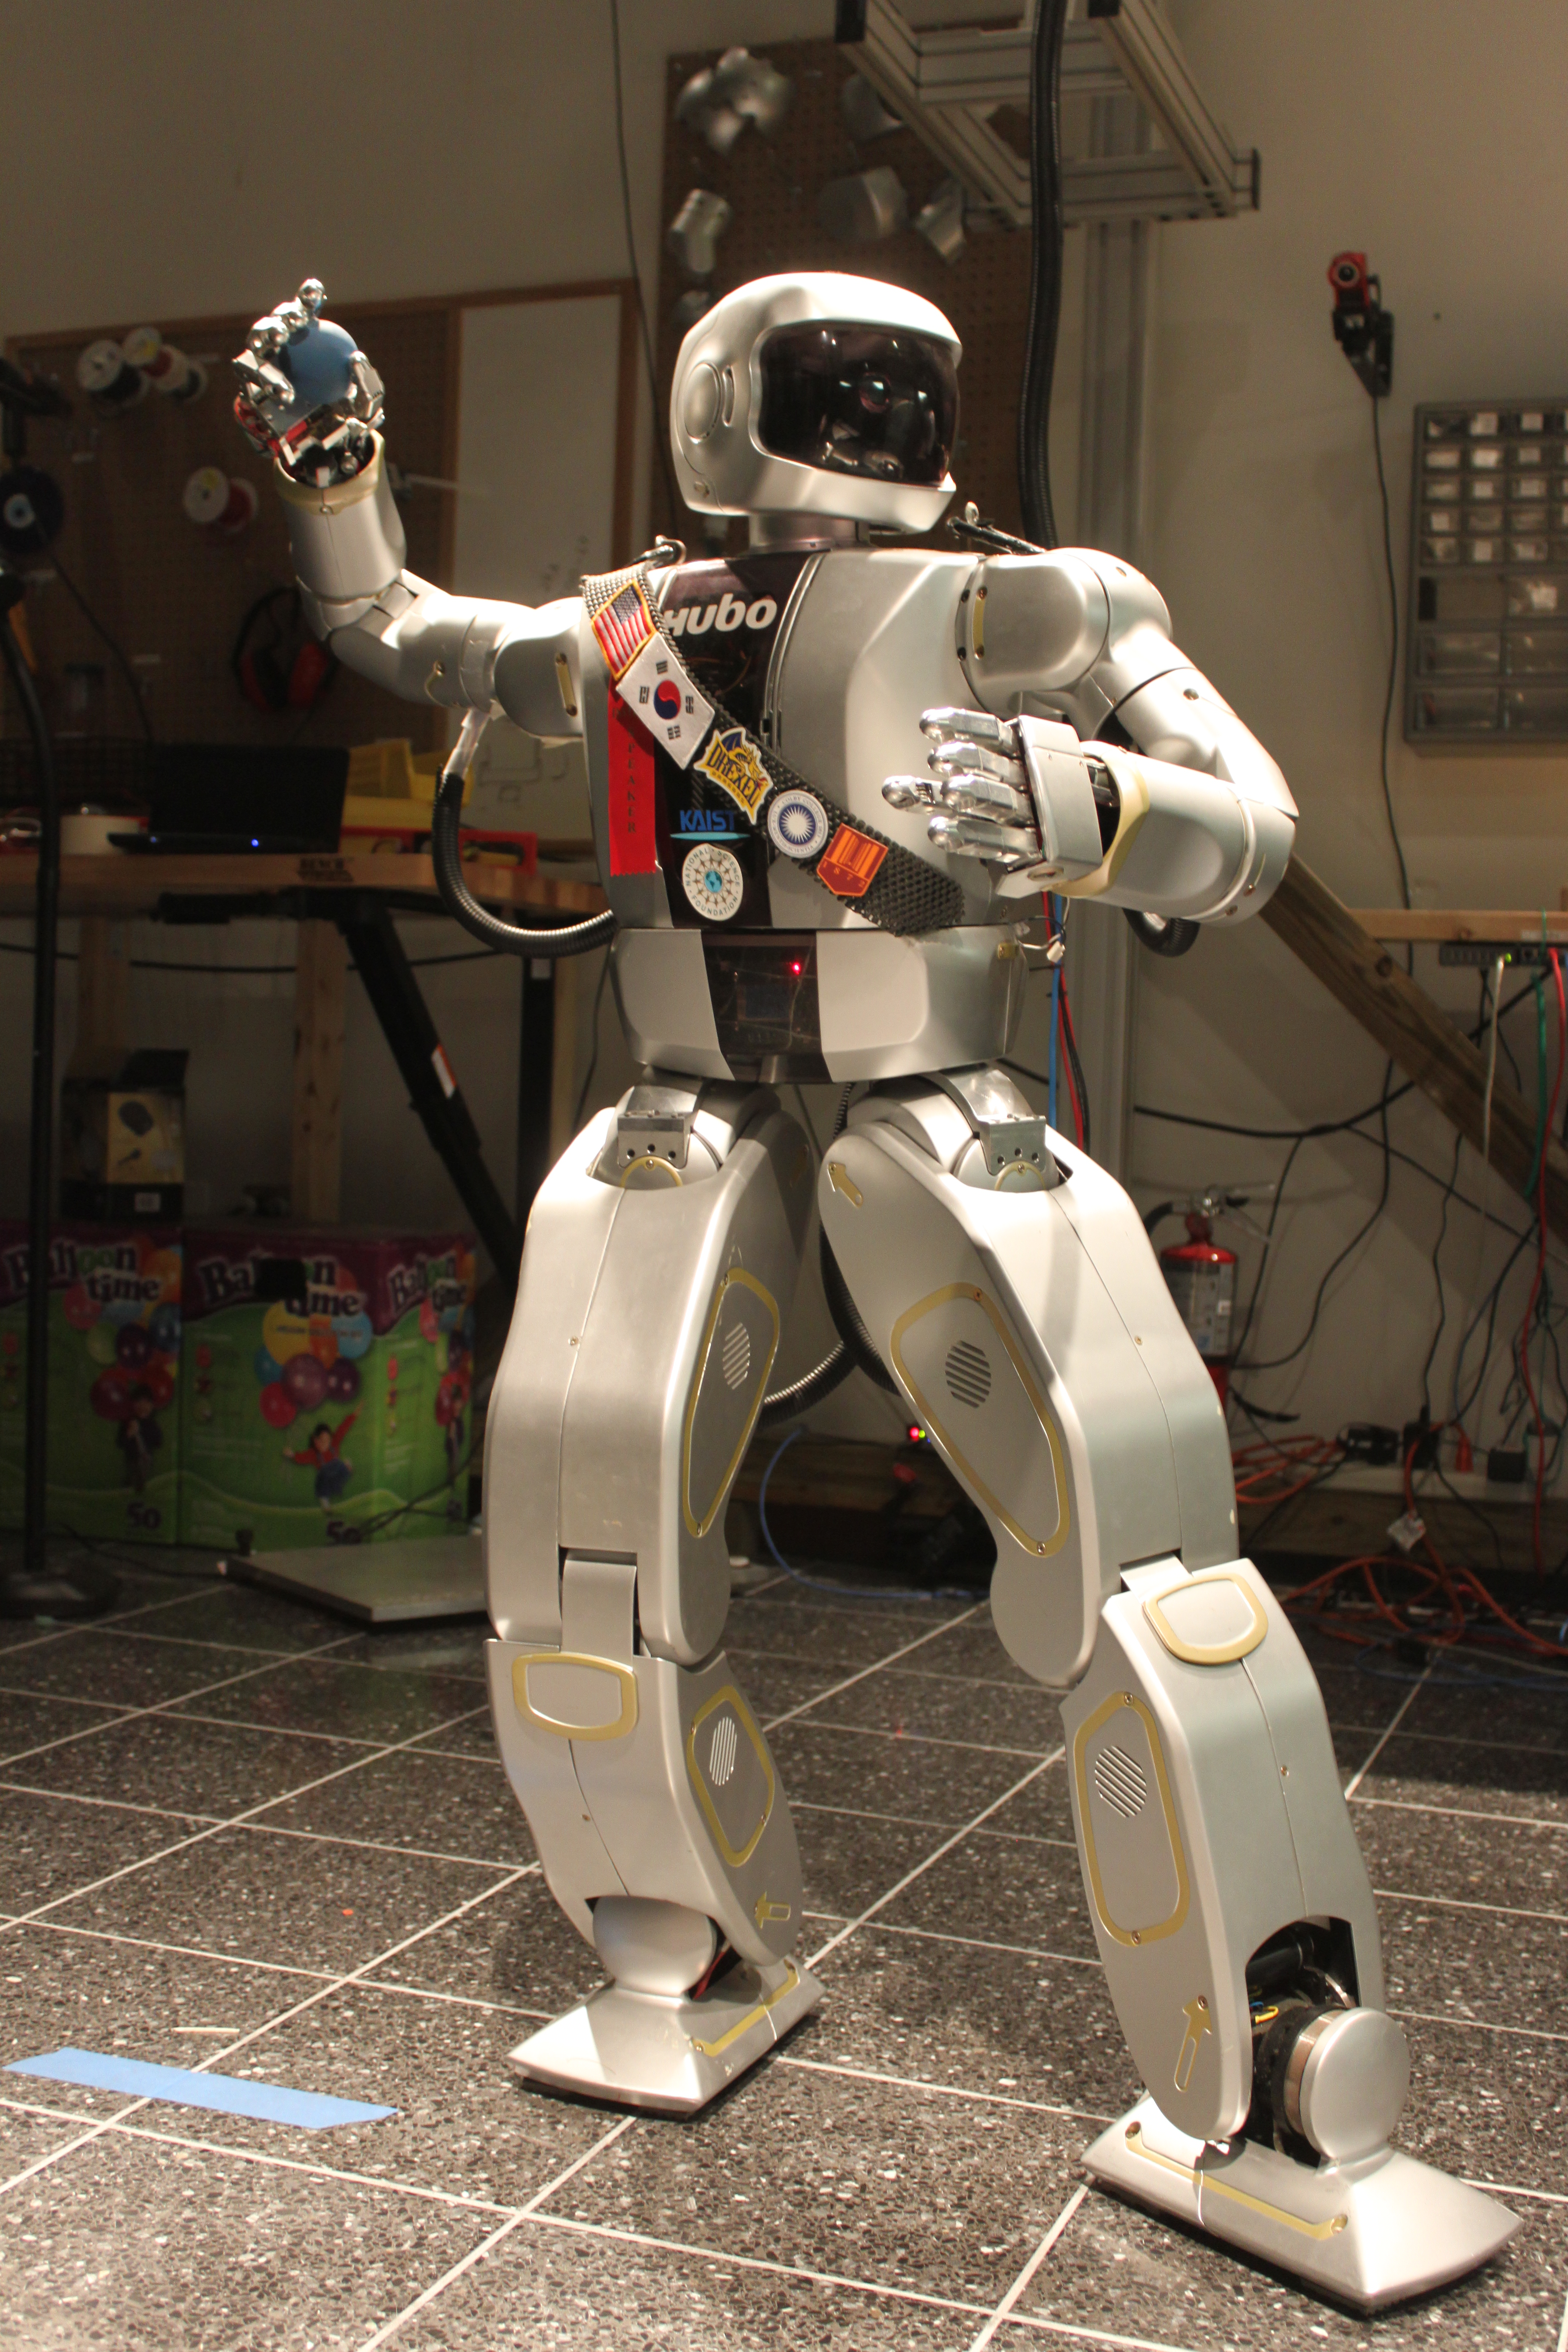
\includegraphics[width=1.0\columnwidth]{./pictures/huboThrow.png}
  \caption{Jaemi Hubo (Hubo KHR-4): The 130cm, 37kg adult size humanoid robot made by Dr. Jun-Ho Oh, director of the Hubo Lab at the Korean Advanced Institute of Science and Technology (KAIST).  Jaemi has been located at the Drexel Autonomous Systems Lab (DASL) at Drexel University since Fall of 2008.}
  \label{fig:huboOneFoot}
\end{figure}

Mechanisms with only a single degree of freedom are restricted to throwing in a plane.   2-DOF mechanisms are able to throw in $R^3$ space with the correct kinematic structure.  Such a mechanism can choose its release point or its end-effector velocity but not both.  Mechanisms containing 3 or more DOF with the correct kinematic structure are able to throw in $R^3$ and choose both the release point and the end-effector velocity.  

Low degree of freedom throwing machines/robots are common.  Typical throwing robots have between one and three degrees of freedom (DOF) \cite{509405, Lynch97dynamicnonprehensile, 5152525, 509335, springerlink:10.1007/s10015-006-0401-0}.  All of these mechanisms are limited to throwing in a plane.   Sentoo et al.\cite{4651142} achieved an end-effector velocity of 6.0 m/s and can throw in $R^3$ space using it's Barret Technology Inc 4-DOF arm with a $360^o$ rotation base yaw actuator.  These low degree of freedom throwing robots are either physically attached/planted to the mechanical ground or have a base that is significantly more massive then the arm.  

Haddadin et al.\cite{6094757} used their 7-DOF arm and a 6-DOF force torque sensor and standard feedback methods to dribble a basket ball.  In addition Zhikun et al.\cite{6094892} used reinforcement learning to teach their 7-DOF planted robot arm to play ping-pong.  Likewise Schaal et al.\cite{schaal01/BIRG} taught their high degree of freedom (30-DOF) humanoid robot to hit a tennis ball using on-line special statistical learning methods.  Visual feedback was used in the basketball throwing robot by Hu et al. achieving accuracy an of 99\%~\cite{5649335}.  All of the latter robots were fixed to the ground to guarantee stability.

Kim et al. \cite{5686315,JooH2011438} takes the research to the next level with finding optimal overarm and sidearm throwing motions for a high degree of freedom humanoid computer model.  The model consists of 55-DOF and is not fixed to mechanical ground or a massive base.  Motor torques are then calculated that allows for both a sidearm or overarm throw and continuously satisfies the zero-moment-point stability criteria\cite{4309277}.  

The highly articulated 40-DOF adult size humanoid robot Jaemi Hubo KHR-4 (Fig.~\ref{fig:huboOneFoot}) is the platform focused on in this work.  Jaemi Hubo is a high-gain, position-controlled biped humanoid robot weighing 37kg and standing 130cm tall.  It is designed and made by Dr. Jun-Ho Oh director of the Hubo Lab at the Korean Advanced Institute of Science and Technology (KAIST).  Jaemi has been located at the Drexel Autonomous Systems Lab (DASL) at Drexel University since Fall of 2008.  DASL has extensive experience with the Jaemi Hubo KHR-4 platform in full body locomotion\cite{5686276}, humanoid control systems\cite{5686325}, full and quarter scale surrogate testing platforms\cite{5379582}, and human robot interaction\cite{5686847,6094987,5928689}.


%  The end-effector position at the desired velocity does not need to be specified.
	
% \section{RELATED WORK}
%	\section{RELATED WORK}

Low degree of freedom throwing machines/robots are common.  Typical throwing robots have between one and three degrees of freedom (DOF) \cite{509405, Lynch97dynamicnonprehensile, 5152525, 509335, springerlink:10.1007/s10015-006-0401-0}.  All of these mechanisms are limited to throwing in a plane.   Sentoo et al.\cite{4651142} achieved an end-effector velocity of 6.0 m/s and can throw in $R^3$ space using it's Barret Technology Inc 4-DOF arm with a $360^o$ rotation base yaw actuator.  These low degree of freedom throwing robots are either physically attached/planted to the mechanical ground or have a base that is significantly more massive then the arm.  

%\cite{5686315,JooH2011438}
Kim et al. \cite{JooH2011438} takes the research to the next level with finding optimal overarm and sidearm throwing motions for a high degree of freedom humanoid computer model.  The model consists of 55-DOF and is not fixed to mechanical ground or a massive base.  Motor torques are then calculated that both allows for a sidearm or overarm throw and continuously satisfies the zero-moment-point stability criteria\cite{4309277}.  

%Kim was able to receive a maximum flight time of 2.784s and 3.711s for overarm and sidearm throws respectively.



	
	
% \section{METHODOLOGY}
	\section{METHODOLOGY}\label{sec:methodology}
To create a valid throwing trajectory for a high-DOF, high-gain, position controlled robot, a desired line in $R^3$ in the direction of the desired velocity must be created.  Each point in the line are temporally separated by the robot's command period $T_r$.  All points in this line must be reachable.  Each point in the line must have a poses that does not create a self collision.  A valid throwing trajectory is created when the latter criteria are met.

\subsection{Self Collision Detection}\label{sec:selfCollision}
Self collision is an important when dealing with a high degree of freedom robot.  Unwanted self collisions can cause permanent damage to the physical and electrical hardware as well as causing the robot not to complete the given task.

To aid in the detection of self collisions a detailed model of the Hubo KHR-4 was made in the widely used open-source robot simulation environment OpenRAVE\cite{diankovThesis}.  The model was created by exporting the three dimensional schematics that the physical robot was created with, to a format that OpenRAVE can use.  This was done in order to ensure an accurate and detailed model.  For these experiments we needed the external boundaries only; the internal geometry was replaced with a simplistic representation.  The external shell is the only part now visible, see Fig~\ref{fig:vHubo} (Left).  The Proximity Query Package (PQP) was used to detect collisions between any two pieces of the robot's external shell.  Due to the high polygon count of the external shell the computation time of detecting a collision was on the magnitude of seconds.  It is advantageous to reduce this time if the system is to run live on the robot.  Computation time is decreased significantly when boundary/collision geometries are simplified due to the lower polygon count.  The collision geometries were further simplified to decrease computation time by making them primitives such as spheres, cylinder and boxes, see Fig~\ref{fig:vHubo} (Right). 

\begin{figure}[thpb]
  \centering
%\includegraphics[width=0.5\columnwidth]{./pictures/hubo1s.png}\includegraphics[width=0.5\columnwidth]{./pictures/hubo2s.png}
\includegraphics[width=0.5\columnwidth]{./pictures/final/hBody.png}\includegraphics[width=0.5\columnwidth]{./pictures/final/hCol.png}
  \caption{OpenRAVE model of Hubo KHR-4. Left: Model with protective shells.  Right: Collision Geometry  }
  \label{fig:vHubo}
\end{figure}

Joint limitations are added to the model to mimic the physical robot.  The model can be commanded the same configurations as the physical robot.  A pose is commanded to the model, PQP searches for any collisions.  With the simplified collision geometry self collisions are detected on the order of milliseconds.  If there are no collisions then the pose can be applied to the physical robot.  A 5\% increase in volume between the simplified collision geometry and the high polygon geometry was added to ensure all of the physical robot's movements will not collide due to minor calibration errors.


\subsection{Reachable Area}\label{sec:rarea}
The desired end effector velocity must be achieved with all joint limits and self-collision constraints satisfied at all times. Typical methods of determining reachability is to move each joint through its full range of motion for each degree of freedom\cite{100034,springerlink:101007}. Due to the high degree of freedom of the Hubo KHR-4 this method is not desirable.  A sampling method described in this work is similar to Geraerts et al.\cite{1570152}.  It was used to accommodate the high degree of freedom system.

The active and the static joints must be defined to calculate the reachable area of a manipulator at a discrete time $N$.  The static joints are assumed to hold a fixed position at time step $N$.  Active joints are free to move to any position as long as it satisfies the joint angle limitations and does not create a self collision.  A uniform random number generator is used to assign each active joint with an angle in joint space.  Each random angle assigned is within the valid range of motion of the respective joint.  The self collision model described in Section~\ref{sec:selfCollision} is used to determine the self collision status with the randomly assigned joint angles.  If there is no self collision the end-effector position and transformation matrix $T$ are calculated using forward kinematics.

\begin{equation}\label{eq:fk1}
\mathbf{
\chi_i = \begin{bmatrix} R_{i} & \Gamma_{i} \\ 0 & 1 \end{bmatrix}
}
\end{equation}

\begin{equation}\label{eq:fk2}
T = \chi_1 \cdot \chi_2 \cdot ... \cdot \chi_n
\end{equation}
%\chi = \begin{bmatrix} R & \left[ \begin{array}{c} x \\ y \\ z \right]\end{array} \\ \left[ \begin{array}{cc} 0 & 0 & 0 & 1 \end{array} \right]  \end{bmatrix} 
%\chi = \begin{bmatrix} xz & xw \\ yz & yw \end{bmatrix} = \left[ \begin{array}{c} x \\ y \end{array} \right] \times \left[ \begin{array}{cc} z & w \end{array} \right] 
%\chi = \begin{bmatrix} R & T \\ 0 & 1 \end{bmatrix}
Where $\chi_i$ is the transformation between joint $i-1$ and $i$, $R_i$ is the rotation of joint $i$ in respect to joint $i-1$ and $\Gamma_i$ is the translation of joint $i$ in respect to joint $i-1$, and $n$ is the number of joints in the kinematic chain.

The end effector position and the joint angles used are recorded.  This process is repeated multiple times to form a sparse representation of reachable end-effector positions in $R^3$ and the corresponding joint angles in joint space.  The resulting representation is called the Sparse Reachable Map (SRM).  Fig.~\ref{fig:sparseRegion} shows that the valid end-effector locations of the right arm between -0.40m and 0.40m on X, -0.40m and 0.40m on Z, and -0.21 to -0.22m on Y.  Fig.~\ref{fig:vHuboSparse} shows the SRM of the entire right arm.  The SRM is used to calculate valid movement trajectories.


\begin{figure}[thpb]
  \centering
\includegraphics[width=1.0\columnwidth]{./MATLAB/reachable2DofR4p8.pdf}
  \caption{Sparse region of reachable locations for the robot's right arm between -0.40m and 0.40m on X, -0.40m and 0.40m on Z, and -0.21 to -0.22m on Y.  Region created by randomly sampling from joint space.  All shown points are valid kinematic solutions that do not cause a self collision.}
  \label{fig:sparseRegion}
\end{figure}

\begin{figure}[thpb]
  \centering
%\includegraphics[width=0.5\columnwidth]{./pictures/hubo1s.png}\includegraphics[width=0.5\columnwidth]{./pictures/hubo2s.png}
\includegraphics[width=0.5\columnwidth]{./pictures/final/SRM.png}\includegraphics[width=0.5\columnwidth]{./pictures/final/ThrowTrajDiag.png}
  \caption{OpenRAVE model of Hubo KHR-4. Left: Model with SRM of right arm.  Right: SRM (blue) with setup and velocity phase trajectories (green)  }
  \label{fig:vHuboSparse}
\end{figure}



\subsection{Trajectory Generation}\label{sec:trajGen}
An end-effector velocity, $V_e$, is chosen based on target location, the well known equations of projectile motion, and the required velocity duration $t_e$.  $V_e$ must be held for a time span of $t_e$, the release point must be within the time span $t_e$.  The magnitude of the velocity in the direction of $V_e$ immediately preceding time span $t_e$ must be less then or equal to the magnitude of $V_e$ during $t_e$.  $t_e$ must be an integer multiple of the robot's actuator command period $T_r$.

A line, $L_d$, in $R^3$ is created with the origin $(x_0, y_0, z_0)$ in the direction of $V_e$.  Each subsequent point in the line $(X_1, Y_1, Z_1)$, $(X_2, Y_2, Z_2)$ $\cdots$ $(X_n, Y_n, Z_n)$ are separated by a time span $T_r$.

The desired velocity is defined as

\begin{equation}
V_e = V_xi+V_yj+V_zk
\end{equation}

%\begin{equation}
%|V_e| =  \sqrt{V_x^2i+V_y^2+j+V_z^2k}
%\end{equation}

%\begin{equation}
%|L_d(N)_n^{n+1}| = \frac{\sqrt{\Delta X^2i + \Delta Y^2j + \Delta Z^2k}}{T_r}
%\end{equation}

%\begin{equation}
%\Delta L_d(N)_n^{n+1} = \frac{\Delta Xi + \Delta Yj + \Delta Zk}{T_r}
%\end{equation}

The line $L_d$ is defined as

\begin{equation}
L_d(n) = X_ni + Y_nj + Z_nk
\end{equation}

Where $n$ is the current zero based time step index value for the time span $t_e$.  The change between time step $n$ and $n+1$ in respect to time of $L_d$  must be equal to our desired velocity $V_e$.

%\begin{equation}
%\Delta L_d(N)_n^{n+1} = \Delta Xi + \Delta Yj + \Delta Zk
%\end{equation}

\begin{equation}
\frac{\Delta L_d|_n^{n+1}}{T_r} = V_e
\end{equation}

\begin{equation}
V_di+V_dj+V_dk = \frac{\Delta Xi + \Delta Yj + \Delta Zk}{T_r}
\end{equation}

Break up into its $i$, $j$, and $k$ components.

\begin{eqnarray} 
V_di & = &  \frac{\Delta Xi}{T_r}  =  \frac{X_{n+1} - X_n}{T_r}\\
V_dj & = &  \frac{\Delta Yi}{T_r}  =  \frac{Y_{n+1} - Y_n}{T_r}\\
V_dk & = &  \frac{\Delta Zi}{T_r}  =  \frac{Z_{n+1} - Z_n}{T_r}
\end{eqnarray}

Solve for the current step $n$ in terms of the origin $(X_0, Y_0, Z_0)$

\begin{eqnarray} 
X_n & = & n(V_di \cdot T_r) + X_0  \\
Y_n & = & n(V_dj \cdot T_r) + Y_0  \\
Z_n & = & n(V_dk \cdot T_r) + Z_0  
\end{eqnarray}

The line $L_d$ can now be defined in terms of the origin $(X_0, Y_0, Z_0)$ and the current zero based time step index value $n$.

\begin{equation}
L_d(n) = n \cdot V_d \cdot T_r + L_d(0)
\end{equation}


Where 

\begin{equation}
L_d(0) = (X_0, Y_0, Z_0)
\end{equation}

%\begin{eqnarray} 
%L_d(n) 	&	= &	(n \cdot V_x \cdot T_r + X_0)i   \\  
%				&	  & + (n \cdot Y_x \cdot T_r + Y_0)j   \\
%				&   & + (n \cdot Z_x \cdot T_r + Z_0)k
%\end{eqnarray}

%\begin{equation} 
%L_d(n) 		= 	(n \cdot V_di \cdot T_r + X_0)i    
%				 + (n \cdot V_dj \cdot T_r + Y_0)j   	
%				 + (n \cdot V_dk \cdot T_r + Z_0)k
%\end{equation}

The line $L_d$ trajectory that the robot's end effector must follow during the time span $t_e$.  A starting point $L_d(0)$ must be found so that $L_d$ is within the reachable area.  $L_d(0)$ is set to a random starting points chosen within the within SRM.  

\begin{equation}
L_d(0) \in SRM
\end{equation}

All subsequent points in $L_d$ must fall within some Euclidean distance $d$ from any point in SRM.  If one of the points in $L_d$ fails this criteria a new random point is chosen for $L_d(0)$ and the process is repeated. 

Once an $L_d$ is found that fits the above criteria the inverse kinematic solution must be found for each point and checked for reachability.  Smaller values of $d$ will increase the probability $L_d$ is within the reachable area defined in the SRM however more iterations will be required to find a valid $L_d$.  Larger values of $d$ will decrease the number of iterations needed to find a valid $L_d$ however the probability of $L_d$ being in the reachable area is decreased.  In addition larger values of $d$ decreases the system's ability to properly map near sharp edges in the SRM.  Increasing the number of samples in the SRM will allow for larger values for $d$.

\subsection{Inverse Kinematics}\label{sec:ik}
The trajectory $L_d$ has one point with a known kinematic solution in $R^3$ and in joint space, $L_d(0)$.  The joint space kinematic solutions for points $L_d(1) \rightarrow L_d(n)$ are unknown.  Mapping the robot's configuration $q \in Q$ to the desired end-effector goal $x_g \in X$, where $Q$ is the robot's configuration space and $X$ is in $R^3$, is done using Jacobian Transpose Controller used by Weghe et al.\cite{4813913}.  Weghe shows the Jacobian as a linear map from the tangent space of $Q$ to $X$ and is express as

\begin{equation}
\dot{x} = J\dot{q}
\end{equation}

  The Jacobian Transpose method is used because of the high DOF of the Hubo KHR-4.  Under the assumption of an obstacle-free environment the Jacobian Transpose Controller is guaranteed to reach the goal.  A proof is shown by Wolovich et al.\cite{4048118}.

To drive the manipulator from its current position $x$ to the goal positions $x_g$ the error $e$ is computed and the control law is formed.

\begin{equation}
e = x_g - x
\end{equation}

\begin{equation}
\dot{q} = kJ^Te
\end{equation}

Where k is a positive gain and self collisions are ignored.  The instantaneous motion of the end-effector is given by

\begin{equation}
\dot{x} = J\dot{q} = J(kJ^Te)
\end{equation}

The final pose $q$ for our goal position $x_g$ can now be found.

The Jacobian Transpose method works best when there is a small difference between the current position $x$ and the goal position $x_g$.  $L_d(0)$ is known both in $X$ and in $Q$ and is the starting point.

\begin{equation}
x = L_d(0)
\end{equation}

\begin{equation}
q_0 = SRM  \left( L_d(0) \right)
\end{equation}

The goal position $x_g$ is set to the next point in $L_d$

\begin{equation}
x_g = L_d(1)
\end{equation}

The pose $q_1$ can now be calculated

\begin{equation}
q_1 = q_0 + \dot{q}_0 = q_0 + kJ^Te|_{x}^{x_g}
\end{equation}

Where $x_g = L_d(0)$ and $x = L_d(1)$.  $L_d(1)$ is now known both in $X$ and in $Q$.  Now $x = L_d(1)$ and the process is repeated until all points in $L_d$ are known both in $X$ and in $Q$.




\begin{figure}[thpb]
  \centering
\includegraphics[width=1.0\columnwidth]{./MATLAB/throwTraj3D.pdf}
  \caption{Sparse Reachable Map Cross Section for Right Arm with setup phase and velocity trajectory $L_d$ }
  \label{fig:3dThrowPlot1}
\end{figure}

\subsection{On-Line Trapezoidal Motion Profile}\label{sec:trap}

The robot's starting position $\vec{x}_0$ is not guaranteed to be the same as the
first point in the velocity trajectory $\vec{L}_d$.  To avoid over large
accelerations when giving this step input from $\vec{x}_0$ to $L_d(0)$ an on-line
trapezoidal motion profile (TMP) was used to generate joint space commands with
the desired limited angular acceleration and velocity.  The TMP was only active
during the setup phase where the robot's end-effector moves from $\vec{x}_0$ to
$L_d(0)$.  This is because the TMP's inherent nature has the potential to adversely effect the desired velocity in $R^3$ under high angular velocity and acceleration conditions in joint space.

The TMP was designed to limit the applied angular velocity and acceleration in
joint space and to prevent over-current/torque. An important advantage over
simply limiting output velocity and acceleration is that the TMP has little to
no overshoot. When a clipped and rate-limited velocity profile is integrated,
the resulting position trajectory may over or undershoot due to this non-linear
system behavior.  The TMP accounts for the imposed limits inherently, and will
arrive at a static goal without overshoot.  Table~\ref{table:trap} describes the three regions
that make up the TMP.
%TODO: Several statements in here are a bit conjectural

%There are three major steps from the initial state to a goal position:
%(1) Accelerate at maximum acceleration in the direction of the goal
%(2) Achieve and hold maximum velocity
%(3) Decelerate to zero velocity to reach goal

\begin{table}[h]
\centering
\caption{Trapezoidal Motion Profile Regions}
\begin{tabular}{|l||l|}
\hline
Region 1	&	Accelerate at maximum acceleration in direction of goal \\ \hline
Region 2	& Achieve and hold maximum velocity \\ \hline
Region 3 	& Decelerate to zero velocity to reach goal \\ \hline
\end{tabular}

\label{table:trap}
\end{table}


%\begin{enumerate}
%\item Accelerate at maximum acceleration in the direction of the goal
%\item Achieve and hold maximum velocity
%\item Decelerate to zero velocity to reach goal
%\end{enumerate}

The area under the velocity trapezoid is the total displacement achieved by the
profile. By shaping this profile based on initial and goal conditions, any
goal position can be precisely reached, even if velocity clipping occurs. The
shape of the profile can be challenging to identify, since it is not
always a trapezoid. For small displacements and large velocity and acceleration
limits, the profile will only reach a fraction of maximum velocity, and will be
triangular. The varying shape of the profile means that calculating and storing
the entire profile for each update could be computationally expensive. 
%THis is a weak statement, since I can't back that up.  Really, it's just unncecessary since my way is better.

The area under the trapezoid can be divided into an accelerating
\eqref{eq:trapslope} and constant velocity portions, where the area is simply a
triangle. The time to accelerate is solved from the final velocity and the
acceleration limit

\begin{equation}
\label{eq:trapslope}
\Delta x=\frac{v_{max}\tau}{2}=\frac{v_{max}^2 sign(v_{max})}{2a_{max}}
\end{equation}

An important consequence of this calculation is that all trapezoidal profiles
end by decelerating at the acceleration limit to the goal position. Rewriting
\eqref{eq:trapslope} slightly, the deceleration (stopping) distance $d_s$ can be found
from the current velocity $v_0$ in \eqref{eq:decdist}. As long as the goal
distance and deceleration distance are equal, then the controller simply
needs to decelerate at the maximum rate to come to rest at the goal.
Conversely, for the current goal distance, there is a critical velocity $v_c$
such that, if the joint began moving at this velocity in the following
timestep, it could decelerate at the maximum rate to reach the position goal.
The controller minimize the error between $v_c$ and the output velocity $v$,
at each timestep.

Since the joint is moving with velocity $v_0$ during a current time-step, some
initial distance $d_{i}$ \eqref{eq:xerr} is traveled before the joint can be
affected. Defining $\hat{u}$ as the sign of the distance to the goal, $v_c$ is
related to $\theta_g$ and $\theta_{err}$ quadratically in \eqref{eq:vc2}. This equation
assumes simple trapezoidal integration. Solving for $v_c$ using the quadratic
formula generally produces complex roots due to the possibility of negative
$v_0$ or $\theta_g$.  In \eqref{eq:vcrit}, $v_0\cdot\hat{u}$ is the current velocity
relative to the goal direction, producing a positive term if the signs of both
terms match. This result will always produce a real value for all $v_0$ and
$\theta_g$.
%TODO: Prove this? it should be possible to plot the root as a surface over v_0
%and x_g

\begin{equation}
\label{eq:decdist}
d_s=\frac{v_0^2 sign(v_0)}{2 a_{max}}
\end{equation}

\begin{equation}
\label{eq:xerr}
d_{i}=v_0 \tau + \frac{v_c-v_0}{2}\tau
\end{equation}

\begin{equation}
\label{eq:uhat}
\hat{u}=sign(\theta_g)
\end{equation}

%\begin{equation}
%\label{eq:vc1}
%v_s^2=x_g 2 a_{max}
%\end{equation}

\begin{equation}
\label{eq:vc2}
v_c^2 = 2 a_{max} \left(\theta_g -\theta_{err} \right)
\end{equation}

\begin{equation}
\label{eq:vcrit}
v_c=\hat{u} a_{max} \left(\sqrt{\frac{a_{max} \tau^2 - 4 \hat{u} v_0 \tau+8 |\theta_g|}{4 a_{max}}} - \frac{ \tau }{2}\right)
\end{equation}


%\section{EXPERIMENT}
	\section{EXPERIMENT}\label{sec:exp}
The goal of throwing a projectile was set to 3.0m, the maximum usable distance in the SISTR system as described in Section~\ref{sec:intro}.  The target is placed directly in front of the robot.  Using the SRM the release point for the projectile motion calculations was set to the mean of the right arm's reachable area, 0.8m from the ground in $z$.  This resulted in a throwing velocity of 4.9m/s at $[\Theta, \Psi, \Phi] =[0.0^o,45.0^o, 3.8^o]$.  This velocity was required to be sustained for 0.1sec due to the speed and accuracy of the gripper's release.  This velocity duration and direction forced the trajectory to produce an underhand throwing gesture.  The projectile is a standard racquetball measuring 57mm in diameter and weighting 42.7g.  The light weight racquetball ball was chosen to assist in not causing instability.  $L_d$ and the setup trajectory are created using the method shown in Section~\ref{sec:methodology} and following all specified constraints.  Fig.~\ref{fig:sparseRegion} shows $L_d$ and the setup trajectory plotted within the SRM.

%\begin{figure}[thpb]
%  \centering
%\includegraphics[width=1.0\columnwidth]{./MATLAB/throwTraj3D.pdf}
%  \caption{Sparse Reachable Map Cross Section for Right Arm with setup phase and velocity trajectory $L_d$ }
%  \label{fig:3dThrowPlot1}
%\end{figure}


\begin{figure}[thpb]
  \centering
\includegraphics[width=0.25\columnwidth]{./pictures/ddFinal/vHside1.png}\includegraphics[width=0.25\columnwidth]{./pictures/ddFinal/vHside3.png}\includegraphics[width=0.25\columnwidth]{./pictures/ddFinal/vHside4.png}\includegraphics[width=0.25\columnwidth]{./pictures/ddFinal/vHside5.png}
\includegraphics[width=0.25\columnwidth]{./pictures/ddFinal/vHside6.png}\includegraphics[width=0.25\columnwidth]{./pictures/ddFinal/vHside7.png}\includegraphics[width=0.25\columnwidth]{./pictures/ddFinal/vHside9.png}
  \caption{Jaemi Hubo running throwing trajectory $L_d$ immediately after the setup phase is completed.  $L_d(0)$ is top left.  Frames are read left to right and have a $\Delta t$ of 0.15s}
  \label{fig:fThrow}
\end{figure}



The trajectory was run on Jaemi Hubo with a position command period $T_r$ of 0.01s.  Fig~\ref{fig:3dThrowReal} shows the side profile of the Jaemi Hubo successfully running the trajectory.  The trajectory shown in Fig~\ref{fig:3dThrowReal} is considered an underhand throw, overhand and sidearm throws are also created with this method.

\begin{figure}[thpb]
  \centering
\includegraphics[width=0.25\columnwidth]{./pictures/slowMotion/1.png}\includegraphics[width=0.25\columnwidth]{./pictures/slowMotion/2.png}\includegraphics[width=0.25\columnwidth]{./pictures/slowMotion/3.png}\includegraphics[width=0.25\columnwidth]{./pictures/slowMotion/4.png}
\includegraphics[width=0.25\columnwidth]{./pictures/slowMotion/5.png}\includegraphics[width=0.25\columnwidth]{./pictures/slowMotion/6.png}\includegraphics[width=0.25\columnwidth]{./pictures/slowMotion/7.png}
  \caption{Jaemi Hubo running throwing trajectory $L_d$ immediately after the setup phase is completed.  $L_d(0)$ is top left.  Frames are read left to right and have a $\Delta t$ of 0.15s}
  \label{fig:3dThrowReal}
\end{figure}

During the experiments the actual position of each joint was recorded.  The total time from the start of the setup phase to the end of the velocity phase is 0.31s.



%\section{EXPERIMENT \& RESULTS}
%\section{RESULTS}
	\section{RESULTS}
The system successfully ran generating valid trajectories.    The commanded trajectory produces the desired velocity of 4.9m/s.  The joint position of the physical joints were logged during runtime.  The velocity and acceleration of the end-effector for the commanded trajectory and the recorded runtime log in the velocity phase can be seen Fig~\ref{fig:posPlot}.  The end effector had large accelerations present when run on the physical system.  

\begin{figure}[thpb]\label{fig:velosPlot}
  \centering
\includegraphics[width=1.0\columnwidth]{./MATLAB/throwTrajRSPplot.pdf}
  \caption{Right shoulder pitch commanded and measured motion profile; Position (top), Velocity (middle), Acceleration (bottom).  The is the result of running the trajectory shown in Fig.~\ref{fig:figThrow} and Fig.~\ref{fig:3dThrowReal}}
\end{figure}


The end effector has large accelerations present because some of the actuators are commanded with accelerations and torques beyond the capabilities of the physical actuator.  The angular velocity and acceleration of the right shoulder pitch joint can be seen in Fig.~\ref{fig:velosPlot}.  The large accelerations combined with the inertia of the arm caused the joint to overshoot the commanded position.  This caused over torque on the pitch joint causing the joint to shutdown in slightly less then 10\% of the trials.



\begin{figure}[thpb]\label{fig:posPlot}
  \centering
\includegraphics[width=1.0\columnwidth]{./MATLAB/throwTrajRSPacc.pdf}
  \caption{The velocity and acceleration of the end-effector for the commanded trajectory and the recorded runtime log in the velocity phase; Velocity (top), Acceleration (bottom).  The is the result of running the trajectory shown in Fig.~\ref{fig:figThrow} and Fig.~\ref{fig:3dThrowReal}.}
\end{figure}










%\section{CONCLUSION \& FUTURE WORK}
%\section{CONCLUSION}
	\section{CONCLUSION AND FUTURE WORK}\label{sec:conc}

As the results in Fig.~\ref{fig:svmMap} in Section~\ref{sec:reslts} show the approach presented in this paper was successful for underhand throwing.  This approach also preforms overhand throwing if the velocity direction, duration, and magnitude falls within the SRM.  While not presented in this paper, results of overhand throwing will be presented in future dissemination of this work.  This work is also constructed in such a way that it is easily applicable other low and high DOF robots.

In the end we solved the problem in the direction that we are going in.  The next logical step is to incorporate full body motion and balancing to the velocity trajectory calculations to further advance us towards our overarching goal.


%This work has shown a valid method of creating trajectories to achieve end-effector velocity control for high degree of freedom position controlled robots.  It was shown the full reachable area does not need to be known to achieve the desired velocity if a good collision model of the robot is available.  It was found that the limiting factor was the robot's physical joints.  This system does create trajectories that fall within the actuators' limitations, however this is not guaranteed.  Immediate future work includes creating a system that will guarantee actuator compliance with the generated trajectory.
	
%\section{FUTURE WORK}
%	\input{futurework}

\section{ACKNOWLEDGMENTS}
	Support for this work was provided by a National Science Foundation - Partnerships for International Research and Education grant (\#0730206).
%\cite{tempo}
\bibliographystyle{IEEEtran}
%\bibliographystyle{plain}
\bibliography{throwing}{}




\end{document}
